\documentclass[compress]{beamer}

%--------------------------------------------------------------------------
% Common packages
%--------------------------------------------------------------------------
\usepackage[english]{babel}
\usepackage{pgfpages} % required for notes on second screen
\usepackage{graphicx}
\usepackage{subfigure}
\usepackage{multicol}
\usepackage[normalem]{ulem}

\usepackage{tabularx,ragged2e}
\usepackage{booktabs}
\usepackage{marvosym}

%--------------------------------------------------------------------------
% Load theme
%--------------------------------------------------------------------------
\usetheme{hri}

\usepackage{tikz}
\usetikzlibrary{patterns,shapes,fpu,fit,calc,mindmap,backgrounds,positioning,svg.path}

\tikzset{
  invisible/.style={opacity=0},
  visible on/.style={alt={#1{}{invisible}}},
  alt/.code args={<#1>#2#3}{%
    \alt<#1>{\pgfkeysalso{#2}}{\pgfkeysalso{#3}} % \pgfkeysalso doesn't change the path
  },
}

%% Neat trick to have only one navigation bullet per subsection
%% http://tex.stackexchange.com/questions/64333/one-navigation-bullet-per-subsection-with-subsection-false-in-custom-beamer-them
%\usepackage{etoolbox}
%\makeatletter
%\patchcmd{\slideentry}{\advance\beamer@xpos by1\relax}{}{}{}
%\def\beamer@subsectionentry#1#2#3#4#5{\advance\beamer@xpos by1\relax}%
%\makeatother
%%%%%%%%%%%%%%%%%%%%%%%%%%%%%%%%%%%%%%%

\graphicspath{{figs/}}

% for model of anthopomorphism
\newcommand{\IPA}{{$\mathcal{A}_0$~}}
\newcommand{\SLA}{{$\mathcal{A}_\infty$~}}
\newcommand{\sla}{{\mathcal{A}_\infty}}
\newcommand{\AntMax}{{$\mathcal{A}_{max}$~}}
\newcommand{\antMax}{{\mathcal{A}_{max}}}

% for HATP plans
\newcommand{\hatpaction}[3]{#1\\\textsf{\scriptsize #2,}\\\textsf{\scriptsize #3}}
\newcommand{\stmt}[1]{{\footnotesize \tt  #1}}

% for mutual modelling
\newcommand{\Mmodel}[3]{{\mathcal{M}(#1, #2, #3)}}
\newcommand{\model}[3]{{$\mathcal{M}(#1, #2, #3)$}}
\newcommand{\Model}[3]{{$\mathcal{M}^{\circ}(#1, #2, #3)$}}

% typeset logical concept
\newcommand{\concept}[1]{{\scriptsize \texttt{#1}}}

\newcommand{\backbutton}{\hfill\hyperlink{appendix}{\beamerreturnbutton{Supplementary material}}}
%--------------------------------------------------------------------------
% General presentation settings
%--------------------------------------------------------------------------
\title{From children free play to Robot AI}
\subtitle{on the way to artificial social cognition in HRI}
\date{AAAI Fall Symposium -- AI-HRI Workshop -- {\bf 15 nov. 2017}}
\author{Séverin Lemaignan}
\institute{Centre for Robotics and Neural Systems\\{\bf
Plymouth University}}

%--------------------------------------------------------------------------
% Notes settings
%--------------------------------------------------------------------------
%\setbeameroption{show notes on second screen}
%\setbeameroption{hide notes}

\begin{document}


%%%%%%%%%%%%%%%%%%%%%%%%%%%%%%%%%%%%%%%%%%%%%%%%%%%%%%%%


%%%%%%%%%%%%%%%%%%%%%%%%%%%%%%%%%%%%%%%%%%%%%%%%%%%%%%%%

\maketitle

\begin{frame}<1>[plain,label=whatsnext]{}

    \begin{center}

    \Large
    \bf How to push back the boundaries of social robotics?

    \end{center}
\end{frame}


\imageframe[caption={open, underspecified situations\par complex~social~dynamics\par rich~semantics\par interplay~of~socio-cognitive~functions}]{pr2-baby-3}

%    \begin{itemize}
%        \item open, underspecified situations
%        \item complex social dynamics
%        \item rich semantics
%        \item interplay of several socio-cognitive functions
%    \end{itemize}


{
\paper{Baxter, Lemaignan, Trafton {\bf Workshop on Cognitive Architectures for Social HRI} -- HRI 2016}
\begin{frame}<5>{Surface functions for Social Cognition}
\centering
        \resizebox{!}{0.7\paperheight}{%
            \begin{tikzpicture}[
                    >=latex,
                every edge/.style={<-, draw, very thick}]
        

            \path[small mindmap, 
                level 1 concept/.append style={sibling angle=360/6}, 
                level 2 concept/.append style={sibling angle=60}, 
            concept color=white,text=hriWarmGreyDark]
            node[concept, visible on=<1-5>] {\bf Social\\Cognition in HRI}
            [clockwise from=30]
            child[concept color=hriSec1,text=white] { node[concept] (percept) {Perception of Human's State}
                [clockwise from=120]
                child[concept color=hriSec3Dark,text=white] { node[concept]
                (emotions) {Empathy Emotions} }
                child[concept color=hriSec2Dark,text=white] { node[concept] (attention) {Attention} }
                child[concept color=hriSec2CompDark,text=white] { node[concept] (mmodel) {Inference of mental models} };
            }
            child[concept color=hriSec2Comp,text=white,grow=-45, visible on=<2->] { node[concept] (knowledge) {Social Knowledge} 
                [counterclockwise from=-140]
                child[concept color=hriSec1CompDark,text=white] { node[concept] (soc-rules) {Social rules} }
                child[concept color=hriSec3Comp,text=black] { node[concept] (soc-ctxt) {Social context} }
                child[concept color=hriSec2Dark,text=white] { node[concept] (memory) {Social memory} }
                child[concept color=hriSec3CompDark,text=white] { node[concept] (common-sense) {Common-sense} };
            }
            child[concept color=hriSec3Comp,text=black, grow=-120,visible on=<3->] { node[concept] (comm) {Communication} 
                [counterclockwise from=180]
                child[concept color=hriSec1CompDark,text=white] { node[concept] (dialog) {Verbal} }
                child[concept color=hriSec1Dark,text=white] { node[concept] (non-verbal) {Non-verbal} };
            }
            child[concept color=hriSec3,text=white,grow=180,visible on=<4->] { node[concept] (dynamics) {Interaction Dynamics} 
                [clockwise from=180]
                child[concept color=hriSec2Dark,text=white] { node[concept] (long-term) {Long-term interaction} };
            }
            child[concept color=hriSec2,text=black, grow=120,visible on=<5->] { node[concept] (action) {Performing with humans} 
                [counterclockwise from=80]
                child[concept color=hriSec2CompDark,text=white] { node[concept] {Action, behaviour recognition} }
                child[concept color=hriSec1Dark,text=white] { node[concept] {Intention reading} }
                child[concept color=hriSec3,text=white] { node[concept] (joint-action) {Joint actions} };
            };


        \end{tikzpicture}
    }
\end{frame}
}

\imageframe[caption={yet...}]{pr2-baby-3}

\note{
    Finding the right task is difficult!

    \begin{itemize}
        \item natural interaction $\Rightarrow$ meaningful task
        \item realistic with today's technologies
        \item reproducible and measurable
        \item focused on social cognition
    \end{itemize}
}

%\videoframe[0.56]{figs/freeplay/maud-zoe-pilot-edit.mkv}
\videoframe[0.56]{figs/freeplay/maud-zoe-pilot-edit.mkv?autostart&noaudio}


\begin{frame}{One question}

    \Large
    \centering

    Can sociality emerge from interaction?

    \pause
    \normalsize
    \vspace{2em}

    Both ``emerge'' as \emph{arise from} and ``emerge`` as in \emph{emergent paradigm of
    cognition}!

    \pause

    ``Social cognition arising in interaction''? certainly looks like a situated \&
    embodied view on cognition

\end{frame}

%%%%%%%%%%%%%%%%%%%%%%%%%%%%%%%%%%%%%%%%%%%%%%%%%%%%%%%%

{
    \paper{cited in Lewandowsky and Farrell, {\bf Computational Modeling In
    Cognition}, 2011}
\begin{frame}{A model?}

    Models attempt to \emph{explain}: 
    \begin{quote}
        ``identifying the causes for an event or phenomenon of interest''
    \end{quote}
    \begin{quote}
        ``unifying disparate phenomena''
    \end{quote}

        A model's value is gained from
    \begin{quote}
        ``predicting facts that, absent the theory, would be antecedently
        improbable''
    \end{quote}

    \pause

    ...we will come back to the predictive power of a model of artifical social
    cognition.

\end{frame}
}
%%%%%%%%%%%%%%%%%%%%%%%%%%%%%%%%%%%%%%%%%%%%%%%%%%%%%%%%

\section{Sketching a model}

%%%%%%%%%%%%%%%%%%%%%%%%%%%%%%%%%%%%%%%%%%%%%%%%%%%%%%%%

\begin{frame}{A model of artificial social cognition}

    I postulate {\bf two stages}:

    \begin{enumerate}
        \item building models of others' minds
        \item exploiting these models to socially act:
            \begin{itemize}
                \item prediction, reading others' intentions
                \item adapting own behaviour, alignment
                \item establish join goals
                \item ultimately, performing joint actions
            \end{itemize}
    \end{enumerate}

    \vspace{2em}
    $\rightarrow$ Social analogs of \emph{perception} \& \emph{action}

\end{frame}

%%%%%%%%%%%%%%%%%%%%%%%%%%%%%%%%%%%%%%%%%%%%%%%%%%%%%%%%

{
    \paper{see discussion in Vernon, {\bf Artificial Cognitive Systems: A Primer} 2014}
\begin{frame}{Cognitivist vs Emergent paradigms}

    ``building'', ``exploiting'', ``reading'', ``establishing''... my terminolgy
    denotes a cognitivist approach (`I, the designer of the system, explicitly implement
    these capabilities')

    \pause
    
    Possible `emergent paradigm' rephrasing:

    \begin{enumerate}
        \item developing internal states \emph{connoting} others' minds
        \item perturbing (influencing) actions synthesis with these states
    \end{enumerate}

    \pause

    {\bf Hybrid approaches} are possible -- mapping to ``raw phenomenal experience'' vs
    ``access counciousness''.
\end{frame}
}

%%%%%%%%%%%%%%%%%%%%%%%%%%%%%%%%%%%%%%%%%%%%%%%%%%%%%%%%

{
    \paper{Graziano {\bf Consciousness and the Social Brain} -- 2013}
\begin{frame}[label=attentionschemata]{Modeling others' mind?}
    \large
    In cognitive neurosciences: Graziano's \emph{Attention Schemata Theory}

    \begin{columns}

        \begin{column}{0.5\linewidth}

            \begin{center}
                \includegraphics<1>[width=1.3\columnwidth]{playing_together}
                \includegraphics<2>[width=1.3\columnwidth]{playing_together_gaze}
                \includegraphics<3>[width=1.3\columnwidth]{playing_together_awareness}
                \includegraphics<4>[width=1.3\columnwidth]{playing_together_mutual_awareness}
            \end{center}

        \end{column}

        \begin{column}{0.5\linewidth}

            \only<2>{
                \vspace*{1.5cm}
                Attention is more about {\bf representation} than visual perspective

                \vspace{0.7cm}
                ``Awareness is a construct that represents the attentional state
                of a brain''

            }
            \only<3>{
                \vspace*{1.5cm}
                Graziano's postulate that modelling other's state of awareness
                is {\bf mediated by one's own attentional system}, through joint
                attention
            }
            \only<4>{
                \vspace*{1.5cm}
                    It follows that {\bf joint attention is the process that gives
                    rise to social awareness}
            }

        \end{column}

    \end{columns}

\end{frame}
}

%%%%%%%%%%%%%%%%%%%%%%%%%%%%%%%%%%%%%%%%%%%%%%%%%%%%%%%%

\begin{frame}{Sketching a path forward: mentalizing}

    {\bf Hypothesis 1}: Graziano is right: mental representations are snapshots of
    \emph{awareness}, \emph{awareness} being itself a label for the
    \emph{memory-mediated process of attention}.

    \pause

    {\bf Hypothesis 2}: this can be extended to social cognition. \textbf{Modeling one
    other mental representations equates to taking snapshots of their current
    state of awareness}.

    As we do not have direct access to others' process of attention, it has to
    be mediated. Following Graziano, we hypotesise that \textbf{modelling other's
    state of awareness is mediated by one's own attentional system, through
    joint attention mechanisms}.


\end{frame}

%%%%%%%%%%%%%%%%%%%%%%%%%%%%%%%%%%%%%%%%%%%%%%%%%%%%%%%%


\section{Free play}


{
    \paper{Parten, {\bf Social participation among preschool children} Journal
    of Abnormal and Social Psychology 1932}
\begin{frame}[label=parten]{Theoretical framework: stages of play}

    In developmental psychology, Parten's {\bf stages of play}:

    \begin{enumerate}
        \item 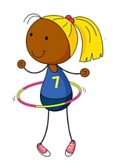
\includegraphics[height=1cm]{figs/stagesofplay/solitary} {\bf Solitary (independent) play}
        \item 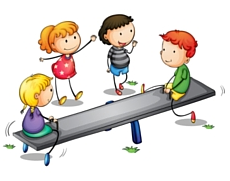
\includegraphics[height=1cm]{figs/stagesofplay/onlooker} {\bf Onlooker play}
        \item 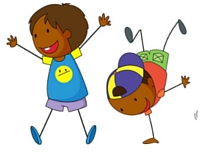
\includegraphics[height=1cm]{figs/stagesofplay/parallel}{\bf Parallel play}
        \item 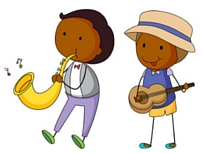
\includegraphics[height=1cm]{figs/stagesofplay/associative}{\bf Associative play}
        \item 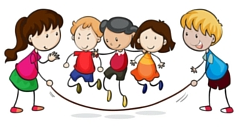
\includegraphics[height=1cm]{figs/stagesofplay/cooperative}{\bf Cooperative play}
    \end{enumerate}

    \note{
    \begin{enumerate}
        \item {\bf Solitary (independent) play}: Playing separately from
            others, with no reference to what others are doing.
        \item {\bf Onlooker play}: Watching others play. May engage in
            conversation but not engaged in doing. True focus on the children at
            play.
        \item {\bf Parallel play} (adjacent play, social coaction): Playing
            with similar objects, clearly beside others but not with them (near
            but not with others.)
        \item {\bf Associative play}:  Playing with others without
            organization of play activity. Initiating or responding to
            interaction with peers. 
        \item {\bf Cooperative play}: Coordinating one’s behavior with that
            of a peer. Everyone has a role, with the emergence of a sense of
            belonging to a group. Beginning of "team work."
    \end{enumerate}
    }


\end{frame}
}

\imageframe[caption=Free-play sandbox]{freeplay/setup}
%\imageframe[color=black]{freeplay/freeplay-sandbox-screenshot}
\imageframe[color=black]{freeplay/analysis}

\note{

    Many dimensions:

    \begin{itemize}
        \item communication
            \begin{itemize}
                \item gaze \& visual attention
                \item social gestures
            \end{itemize}
    \end{itemize}


    Large dataset acquisition: we target about 50 interactions, around 15 min
    each -- two age groups: 4 years old / 7 years old
}

%\videoframe[0.56]{figs/freeplay/zoo-builder-proto-smaller.mkv}

\begin{frame}{A framework for socio-cognitive investigation}

    \begin{center}

    \Large


    \begin{itemize}
        \item {\bf Task-independent social dynamics}\\{\large interaction flow, adaptation,
            social patterns...}
        \item {\bf Situation awareness}\\{\large what happens? who does what?
            why?\\ $\rightarrow$ mind modelling}
    \end{itemize}

    \end{center}

\end{frame}

\begin{frame}{Key outcomes for HRI}

    Real-time identification (and generation?) of...

    \begin{itemize}
        \item the \textbf{interaction flow} (situation awareness)
        \item the \textbf{task engagement}
        \item the \textbf{social behaviours}
            \begin{itemize}
                \item Pro-social, hostile, assertive (‘bossy’), passive...
            \end{itemize}
        \item the \textbf{social dynamics}
            \begin{itemize}
                \item entrainment (coupling), mimicry, turn-taking, joint
                    attention
            \end{itemize}
    \end{itemize}

    \pause
    \begin{itemize}

        \item {\bf emergence of \hyperlink{parten}{Parten's stages of
            play}?}

    \end{itemize}

\end{frame}

\section{Deep learning and robotics}

{
    \paper{Mnih et al. {\bf Human-level control through deep reinforcement learning} -- Nature 2015}
\begin{frame}{Learning Complex Behaviours}

    \begin{center}
        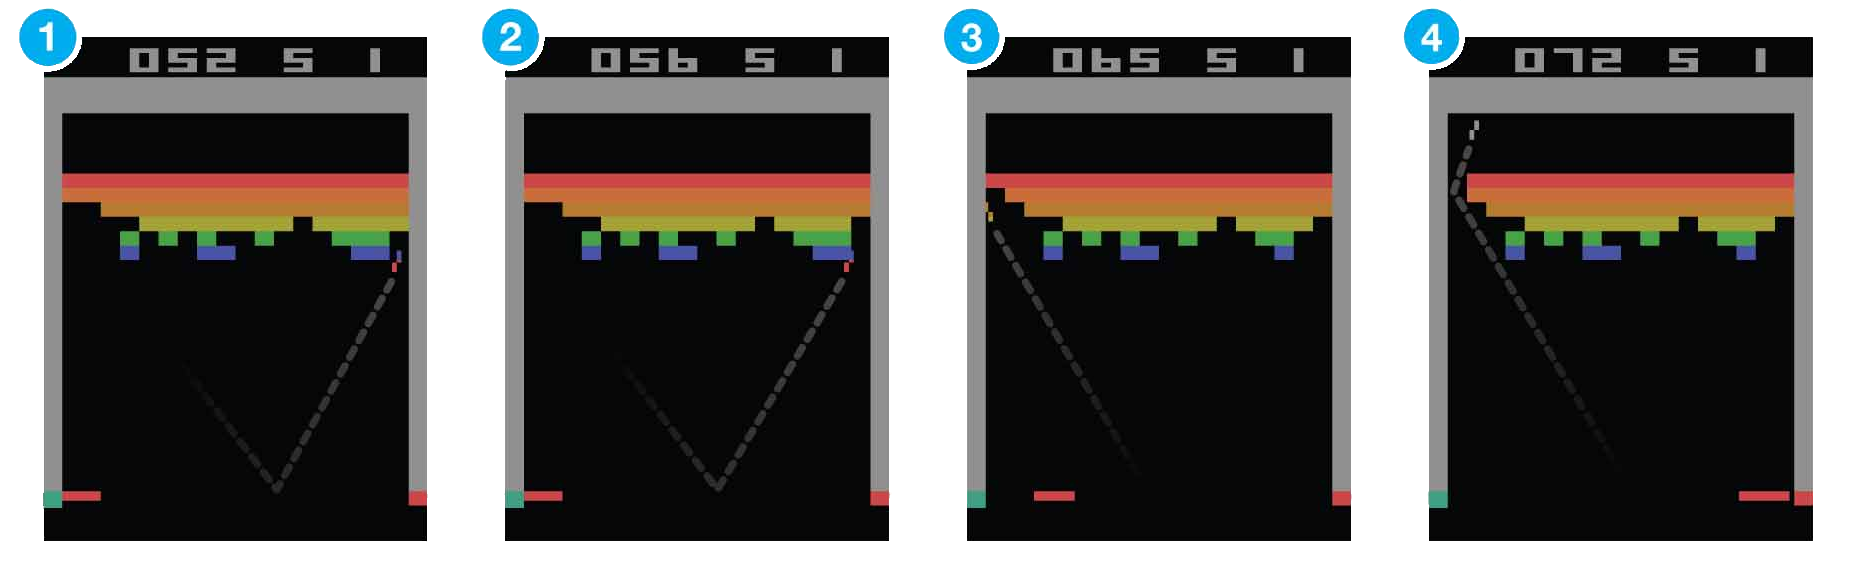
\includegraphics[width=\linewidth]{breakout}
    \end{center}


        \begin{itemize}
            \item Inputs: raw screen image + score
            \item from the outside, looks like planning
            \item<2-> \sout{1.000.000} {\bf 500} games to play a good human-level
        \end{itemize}

    \uncover<3> {
        \begin{center}
            {\bf Could we also learn social dynamics?}
        \end{center}
    }
\end{frame}
}

\videoframe[0.56]{videos/ogata-deeplearning-towel-folding.mp4?autostart&noaudio&start=19}


\section{Deep learning of social interactions?}

{
    \paper{Graziano {\bf Consciousness and the Social Brain} -- 2013] \newline
    [Jaeger {\bf Controlling recurrent neural networks by conceptors} -- 2014}

\begin{frame}{My current vision}

    \begin{center}

    \Large
    \bf (Deep) learning of socio-cognitive human-robot interactions

    \end{center}

    \pause

    \normalsize

    Working hypothesis: \textbf{Sociality emerges from interaction}

%   $\Rightarrow$ situated \& embodied view on social cognition

    \pause

    \begin{itemize}
        \item Instrumental role of \textbf{\hyperlink{attentionschemata}{attention}}
        \item Unsupervised \textbf{recurrent neural networks} to model others'
            minds $\rightarrow$ a \textbf{connectionist theory of mind}

    \end{itemize}

    \pause
    {\bf ...towards a principled model of social cognition?}

\end{frame}
}



\section{PInSoRo}


\begin{frame}{PinSoRo}
 How to push back the boundaries of social
            robotics?

    \begin{itemize}
        \item Open, underspecified situations
            \item complex social dynamics
            \item Natural interactions
            \item rich semantics
            \item interplay of many socio-cognitive functions
    \end{itemize}
        yet,
    \begin{itemize}
        \item Reproducible/replicable situations
        \item Clear quantitative metrics
    \end{itemize}
\end{frame}

\imageframe{freeplay/freeplay-overview}
\imageframe{freeplay/freeplay-overview2}

\imageframe[color=black]{freeplay/3d-point-cloud-facial-features}
\imageframe[color=black]{freeplay/rviz-faces}


\begin{frame}{Main dataset stats}
    \begin{itemize}
        \item 120 children, 4 to 8 years old
     \item 90 children playing with another child, 30 playing with a robot
     \item About 45h+ of child recordings,
     \item average duration of freeplay interactions: 24min in child-child condition,
            19min in child-robot condition
     \item Facial features extracted seen in ~98\% of frames
    \end{itemize}
\end{frame}

\imageframe{freeplay/durations}

\imageframe[scale=0.95]{freeplay/coding-scheme}
\imageframe[scale=0.95, color=black]{freeplay/annotator}
\imageframe[scale=0.95]{freeplay/freeplay-sandbox-architecture}
%%%%%%%%%%%%%%%%%%%%%%%%%%%%%%%%%%%%%%%%%%%%%%%%%%%%%%%%

\imageframe[color=white]{islands1}

%%%%%%%%%%%%%%%%%%%%%%%%%%%%%%%%%%%%%%%%%%%%%%%%%%%%%%%%

\imageframe[color=white]{islands2}

%%%%%%%%%%%%%%%%%%%%%%%%%%%%%%%%%%%%%%%%%%%%%%%%%%%%%%%%

\imageframe[color=white]{islands3}

%%%%%%%%%%%%%%%%%%%%%%%%%%%%%%%%%%%%%%%%%%%%%%%%%%%%%%%%

\imageframe[color=white]{islands4}

%%%%%%%%%%%%%%%%%%%%%%%%%%%%%%%%%%%%%%%%%%%%%%%%%%%%%%%
%%%%%%%%%%%%%%%%%%%%%%%%%%%%%%%%%%%%%%%%%%%%%%%%%%%%%%%%

{
    \fullbackground[color=black]{eeg}
\begin{frame}[plain]

    \begin{columns}
        \begin{column}{0.6\linewidth}
        \end{column}
        \begin{column}{0.4\linewidth}

\setbeamercolor{hriSec1Demo}{fg=white!70!black}
\begin{beamercolorbox}[wd=\linewidth,ht=6ex,dp=0.7ex]{hriSec1Demo}
    \textbf{Thank you!}
    \vspace{3em}
\end{beamercolorbox}
        \end{column}
    \end{columns}
\end{frame}
}

\end{document}
